\documentclass[10pt,a4paper]{article}

\usepackage[utf8]{inputenc}
\usepackage[english]{babel}
\usepackage[T1]{fontenc}
\usepackage{amsmath}
\usepackage{amsfonts}
\usepackage{amssymb}
\usepackage{graphicx}
\usepackage{lmodern}
\usepackage{hyperref}
\usepackage[left=2.7cm,right=2.7cm,top=2cm,bottom=3cm]{geometry}
\usepackage{verbatim}
\usepackage{xcolor}
\usepackage{url}

\hypersetup{
    colorlinks,
    linkcolor={red!50!black},
    citecolor={blue!50!black},
    urlcolor={blue!80!black}
}

\title{
\includegraphics[scale=1]{Art/otb-logo.png}\\
  Develop with OTB\\
  Updated for OTB-6.2\\
  {\small\url{https://www.orfeo-toolbox.org}}
}

\begin{document}

\maketitle

\tableofcontents

\clearpage

\section{Install OTB}

On all platforms, follow the \textbf{OTB Installation Guide} to
download and install OTB using the self-extracting binary package.

\section{Windows}

This section describes how to set up the environment to develop in C++
on Windows using OTB.

You have two methods to build your projects:
\begin{enumerate}
\item Using windows command prompt (cmd.exe)
\item Visual studio IDE
\end{enumerate}

You need Visual Studio 2015 and CMake for building projects using OTB.

\subsection{Clink (optional)}

Clink add Bash's powerful command line editing in cmd.exe. The tool
can be downloaded free of charge from their GitHub page
\url{https://github.com/mridgers/clink}. This tool is optional for
both development and usage of OTB.  But it is highly recommended to
use it rather than using third party terminal emulator such as git
bash or mobaXterm.

\subsection{Visual Studio 2015}

Visual Studio Community Edition can be downloaded free of
charge. However, you must register to get access to the download
page. We use community edition because it is free of charge. If you
have professional or enterprise edition that will work too. The latest
version is 2017 but you must have Visual Studio 2015 for OTB. 

Download visual studio 2015 from
\url{https://www.visualstudio.com/vs/older-downloads/}

Below you can find screenshots from our visual studio 2015
installation.  The default installation does not include C++ compiler
which are required for building OTB (see figure
\ref{fig:vs2015-custom-install}, figure
\ref{fig:vs2015-select-components} and figure
\ref{fig:vs2015-start-install})

\begin{figure}[!htbp]
  \center
  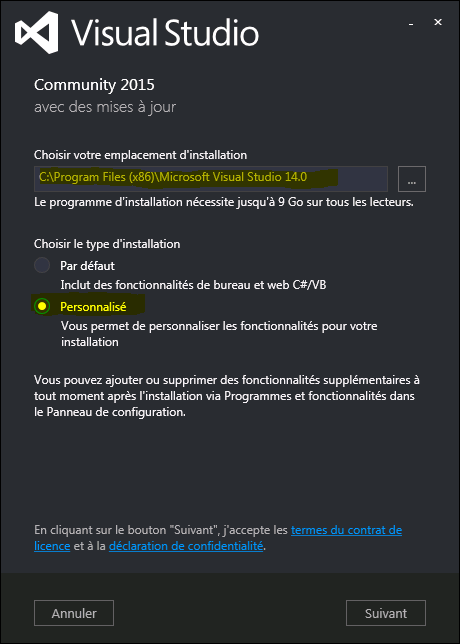
\includegraphics[width=0.7\textwidth]{Art/vs2015-custom-install.png}
  \caption[]{Use custom installation options for VS2015}
  \label{fig:vs2015-custom-install}
\end{figure}

\begin{figure}[!htbp]
  \center
  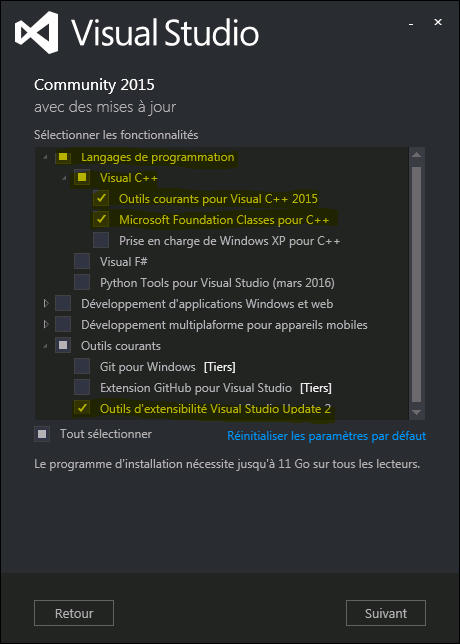
\includegraphics[width=0.7\textwidth]{Art/vs2015-select-components.png}
  \caption[]{Components to select in the VS installation procedure}
  \label{fig:vs2015-select-components}
\end{figure}

\begin{figure}[!htbp]
  \center
  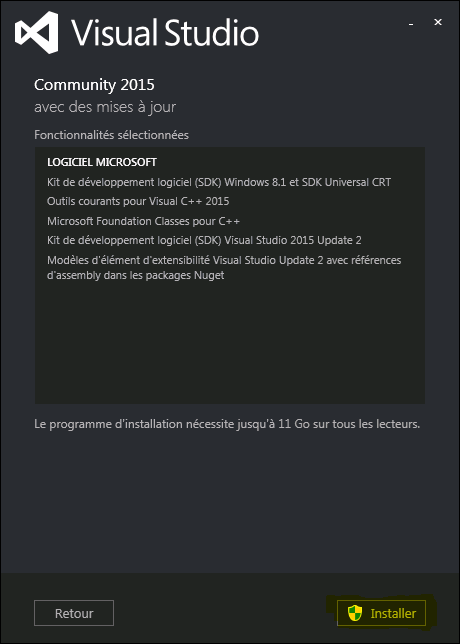
\includegraphics[width=0.7\textwidth]{Art/vs2015-start-install.png}
  \caption[]{Summary of installation option}
  \label{fig:vs2015-start-install}
\end{figure}

\subsection{CMake}

\textbf{CMake is not a required if you are building using the IDE (see section~\ref{ide}).}

CMake installer for Windows can be downloaded from \url{https://cmake.org/files/v3.7/cmake-3.7.2-win64-x64.msi}
\newline
Make sure you add CMake to system PATH (see figure \ref{fig:cmake-install}).

\begin{figure}[!htbp]
  \center
  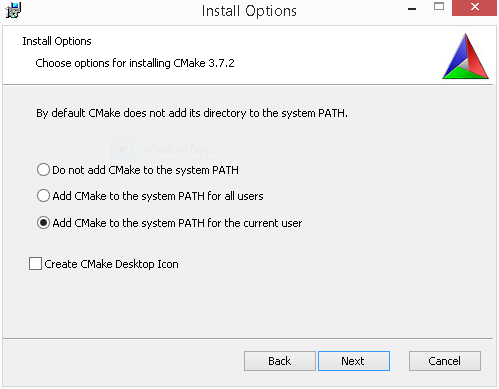
\includegraphics[width=0.7\textwidth]{Art/cmake-install.png}
  \caption[]{cmake-install}
  \label{fig:cmake-install}
\end{figure}

\textbf{CMake is not a required if you are building using the IDE (see section~\ref{ide}).}

\subsection{Develop using windows command prompt}
I've extracted xdk package into \texttt{C:{\textbackslash}projects}. So I will
update variables relative to this path.

\begin{itemize}
  \item Open cmd.exe
  \item The first step is to call \textbf{vcvarsall.bat} from Visual Studio 2015:
  \begin{verbatim}
    call "C:\Program Files (x86)\Microsoft Visual Studio 14.0\VC\vcvarsall.bat" x64
  \end{verbatim}
  \textbf{We assume you had installed visual studio to C: drive} \\
  \textbf{x64 is the machine architecture. For some systems, it is called amd64 or
  x86\_64.}
  \item The next step is to update PATH and CMAKE\_PREFIX\_PATH variables. PATH variable
is required for finding dll files. CMAKE\_PREFIX\_PATH variable is required for
finding packages with cmake configure:
\begin{verbatim}
set PATH=C:\projects\OTB-5.10.1-xdk-win64\bin;$PATH
set CMAKE_PREFIX_PATH=C:/projects/OTB-5.10.1-xdk-win64
\end{verbatim}

\end{itemize}
  
\subsection{Configure and build project}

We can try to build a simple program using cmake to test the
configuration:

\begin{verbatim}
cd c:\projects\otbprojects\build
cmake ..\ex1_HelloWorld -G"NMake Makefiles"
nmake
\end{verbatim}
If build goes fine, you will get executable file HelloWorld.exe
\newline
C:{\textbackslash}projects{\textbackslash}otbprojects{\textbackslash}build{\textbackslash}HelloWorld.exe
\newline

\subsection{Test the Hello World program}

The last step is to run the generated executable:

\begin{verbatim}
> c:\projects\otbprojects\build\HelloWorld.exe
> OTB Hello World !
\end{verbatim}

\subsection{Using Visual Studio IDE}\label{ide}

Please see the wiki page which describes how to set up visual studio project to
develop with OTB:
\url{https://wiki.orfeo-toolbox.org/index.php/Writing_OTB_modules_with_Visual_Studio_IDE}

\clearpage
\section{Linux (Ubuntu example)}

Make sure cmake and gcc (>= 4.9) are installed on your system. You can
print cmake and gcc versions with the following commands: 

\begin{verbatim}
cmake --version
gcc --version
\end{verbatim}

\subsection{Configure and build project}

\begin{verbatim}
cd ~/otbprojects/HelloWorld/
mkdir build
cmake ~/otbprojects/HelloWorld/ex1_HelloWorld -DCMAKE_CXX_FLAGS='-std=c++11'
make
\end{verbatim}

You now have \textasciitilde/otbprojects/HelloWorld/build/HelloWorld

\subsection{Test the Hello World program}

\begin{verbatim}
> ~/otbprojects/HelloWorld/build/HelloWorld
> OTB Hello World !
\end{verbatim}

\section{Mac OS X}

Make sure cmake, and XCode (>= 6.1.1) are installed on your
system. AppleClang is installed with XCode.

Check cmake and gcc version with:

\begin{verbatim}
cmake --version
gcc --version
\end{verbatim}

\subsection{Configure and build project}

\begin{verbatim}
cd ~/otbprojects/HelloWorld/
mkdir build
cmake ~/otbprojects/HelloWorld/ex1_HelloWorld -DCMAKE_CXX_FLAGS='-std=c++11'
make
\end{verbatim}

You now have ~/otbprojects/HelloWorld/build/HelloWorld

\subsection{Test the Hello World program}

\begin{verbatim}
> ~/otbprojects/HelloWorld/build/HelloWorld
> OTB Hello World !
\end{verbatim}

\end{document}
